\chapter{Decyzje projektowe}

\section{Wybór języka Kotlin (Dorota Tomczak)}
\par Przed rozpoczęciem prac implementacyjnych nad projektem należało podjąć decyzję, co do wyboru języka programowania. W przypadku aplikacji mobilnej na system Android, przy założeniu że miałaby to być aplikacja natywna, wybór ten ograniczał się do dwóch opcji – Java lub Kotlin. Ostatecznie zdecydowano o napisaniu aplikacji w Kotlinie, głównie ze względu na fakt, że 7 maja 2019 firma Google na konferencji Google I/O 2019 ogłosiła, że ten język jest obecnie preferowanym językiem do tworzenia aplikacji mobilnych na Androida\cite{Google I/O 2019}. Aby ułatwić jednoczesną pracę nad aplikacją serwerową podjęto decyzję o wykorzystaniu języka Kotlin również i w tym projekcie.
\par Podczas pracy nad projektem oraz z perspektywy czasu po zakończeniu działań implementacyjnych, jednomyślnie stwierdzono, że wybór Kotlina był słuszny. Język ten zapewnia wiele przydatnych udogodnień i ulepszeń w stosunku do języka Java, które wpływają na jakość kodu i satysfakcję z pracy nad nim. Jedną z jego niezaprzeczalnych zalet jest minimalizacja tzw. kodu boilerplate, co przejawia się między innymi w takich jego cechach jak: 

\begin{itemize}
\item utworzenie klasy typu Singleton jest jednoznaczne z dodaniem klasy oznaczonej słowem kluczowym \textit{object},
\item klasy oznaczone słowem kluczowym \textit{data} służące głównie jako obiekty DTO (obiekty wykorzystywane do przesyłania danych), do których to kompilator sam generuje konstruktory oraz metody dostępu do wszystkich pól (rys.~\ref{fig:dtoKotlin}),
\item wyrażenia lambda, czyli w uproszczeniu funkcje anonimowe.
\end{itemize}

\begin{figure}[h]
\centering
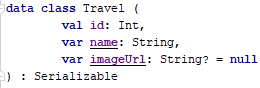
\includegraphics[width=0.7\textwidth]{dtoKotlin}
\caption{Klasa DTO w Kotlinie -- 5 linii kodu.}
\label{fig:dtoKotlin}
\end{figure}
\FloatBarrier

\section{Narzędzia (Magdalena Solecka)}
\subsection{Github}
\par W celu łatwego zarządzania projektem wykorzystano System kontroli wersji \textit{Github}\cite{github}. Repozytorium zawierało trzy foldery: App (zawierający implementację aplikacji mobilnej), ServerApp (zawierający implementację serwera w architekturze REST) oraz Documents (zawierający dokumentację projektu). Backlog produktu utworzono w postaci zadań (ang. issues) również na tej samej platformie (rys.~\ref{fig:github}).  Jako model pracy wybrano \textit{Gitflow}, a jako schemat nazewnictwa gałęzi funkcjonalności (ang. feature branches): \{nr\_zadania\}-skrócona-nazwa-zadania. Również w nazewnictwie zapisów zmian (ang. commits) zdecydowano się na skorzystanie ze wzoru: \#\{nr\_zadania\}: opis wprowadzonych zmian, w celu śledzenia postępów nad danym zadaniem.

\begin{figure}[h]
\centering
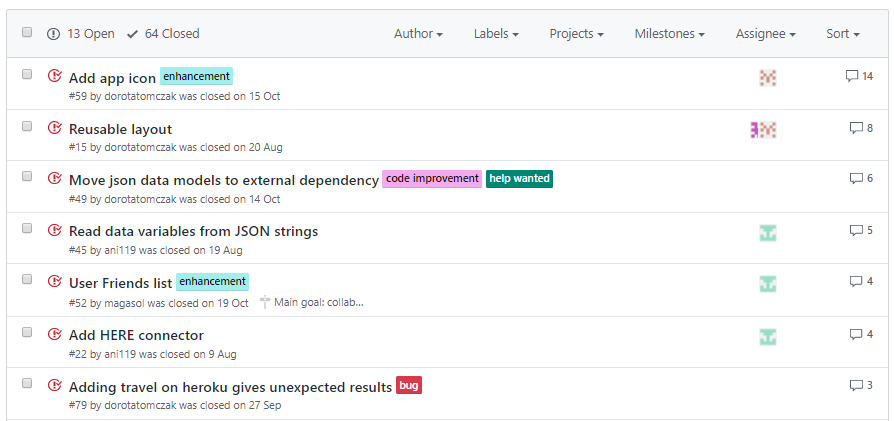
\includegraphics[width=\linewidth]{github}
\caption{Lista zadań implementacyjnych na platformie Github.}
\label{fig:github}
\end{figure}
\FloatBarrier

\subsection{Android Studio i Intellij IDEA}
\par Środowiskiem programistycznym wykorzystywanym podczas implementacji zostały wybrane \textit{Android Studio} dla wytwarzania aplikacji mobilnej i \textit{Intellij IDEA} dla serwera. Są to narzędzia kompatybilne z systemem \textit{Git} co znacznie ułatwiło rozwiązywanie konfliktów podczas pobierania najnowszych zmian ze zdalnego repozytorium. Usprawniło również proces zapisu zmian. Konfiguracje systemów członków zespołu wymagały m.in. wykorzystania różnych portów oraz adresów IP. Praca z systemem \textit{Git} poprzez jeden z programów zamiast konsolę umożliwiała odznaczenie konkretnych linii kodu, więc przy każdym zapisie nie trzeba było ich zmieniać.

\subsection{Heroku}
\par Dla celów testowych oraz prezentacji aplikacji zdecydowano się na wdrożenie projektu na zdalny serwer. Skorzystano z darmowej oferty \textit{Heroku}. Skonfigurowano połączenie pomiędzy repozytorium na platformie \textit{Github} a instancją serwerową na platformie \textit{Heroku} tak, aby po jakiekolwiek zmianie na gałęzi develop następowało automatyczne wdrożenie. W celu poprawnej kompilacji projektu na platformie dodano pakiety: https://github.com/timanovsky/subdir-heroku-buildpack (kompilacja projektu znajdującego się w podkatalogu repozytorium) i heroku/gradle (obsługa Gradle).
